\documentclass[landscape,a0,final]{a0poster}
\usepackage{helvet}
\renewcommand{\familydefault}{\sfdefault}
\usepackage[utf8]{inputenc}
\usepackage[T1]{fontenc}
\usepackage{amsmath,amssymb,amsfonts}
\usepackage{graphicx}
\usepackage{booktabs,colortbl,tabularx,array}
\usepackage{xcolor}
\usepackage[most]{tcolorbox}
\usepackage{tikz}
\usepackage{pgfplots}
\pgfplotsset{compat=1.18}
\usetikzlibrary{positioning,calc,shapes.geometric,backgrounds,patterns,decorations.pathmorphing}
\usepackage{fontawesome5}
\usepackage{enumitem}
\usepackage{microtype}
\usepackage{url}

% Native A0 Landscape Page Dimensions
\setlength{\pdfpagewidth}{118.92cm}
\setlength{\pdfpageheight}{84.10cm}
\setlength{\paperwidth}{118.92cm}
\setlength{\paperheight}{84.10cm}
\setlength{\voffset}{-1in}
\setlength{\hoffset}{-1in}
\setlength{\topmargin}{2.0cm}
\setlength{\oddsidemargin}{2.0cm}
\setlength{\evensidemargin}{2.0cm}
\setlength{\textwidth}{114.92cm}
\setlength{\textheight}{80.10cm}
\setlength{\vsize}{80.10cm}

% Column Types
\newcolumntype{L}[1]{>{\raggedright\arraybackslash}p{#1}}
\newcolumntype{C}[1]{>{\centering\arraybackslash}p{#1}}
\newcolumntype{R}[1]{>{\raggedleft\arraybackslash}p{#1}}
\newcolumntype{Y}{>{\raggedright\arraybackslash}X}

% Custom Palette (2-4 primary colors + neutrals)
\definecolor{NavyDark}{RGB}{15,23,42}
\definecolor{CyanAccent}{RGB}{6,182,212}
\definecolor{BlueAccent}{RGB}{37,99,235}
\definecolor{SlateLight}{RGB}{241,245,249}
\definecolor{CardBg}{RGB}{250,250,250}
\definecolor{BorderColor}{RGB}{203,213,225}
\definecolor{TextDark}{RGB}{30,41,59}
\definecolor{TextMuted}{RGB}{71,85,105}
\definecolor{AmberHighlight}{RGB}{217,119,6}
\definecolor{EmeraldHighlight}{RGB}{16,185,129}
\definecolor{TableHeadBg}{RGB}{30,41,59}

% TColorBox Styles
\tcbset{
  posterbox/.style={
    enhanced,
    colback=CardBg,
    colframe=NavyDark,
    arc=4mm,
    boxrule=2.5pt,
    fonttitle=\large\bfseries\color{white},
    coltitle=white,
    colbacktitle=NavyDark,
    top=8pt,
    bottom=8pt,
    left=10pt,
    right=10pt,
    shadow={2mm}{-2mm}{0mm}{black!15},
    before skip=8pt,
    after skip=8pt
  },
  accentbox/.style={
    enhanced,
    colback=SlateLight,
    colframe=CyanAccent,
    arc=3mm,
    boxrule=2pt,
    fonttitle=\normalsize\bfseries\color{NavyDark},
    coltitle=NavyDark,
    colbacktitle=CyanAccent!20,
    top=6pt,
    bottom=6pt,
    left=8pt,
    right=8pt
  }
}

% Column width definition (4 columns across landscape A0)
\newlength{\colwidth}
\setlength{\colwidth}{0.235\linewidth}

\usepackage{hyperref}
\begin{document}
\setlength{\colwidth}{0.235\linewidth}% recompute against poster \linewidth
\raggedright\emergencystretch=6em\relax
\color{TextDark}

% Reduce math display gaps for poster compactness
\setlength{\abovedisplayskip}{4pt}
\setlength{\belowdisplayskip}{4pt}
\setlength{\abovedisplayshortskip}{2pt}
\setlength{\belowdisplayshortskip}{2pt}

% ==========================================
% HEADER / TITLE BANNER
% ==========================================
\begin{tcolorbox}[
  enhanced,
  colback=NavyDark,
  colframe=CyanAccent,
  arc=6mm,
  boxrule=3.5pt,
  top=12pt,
  bottom=12pt,
  left=18pt,
  right=18pt,
  shadow={3mm}{-3mm}{0mm}{black!25}
]
  \begin{minipage}[c]{0.73\linewidth}
    {\VERYHuge \bfseries \color{white} High-Density Plasma Turbulence \& MHD Transport in Tokamak Divertors} \\[8pt]
    {\veryHuge \bfseries \color{CyanAccent} High-Resolution Langmuir-Doppler Diagnostics and 5-Field Gyrofluid SOL Simulations} \\[12pt]
    {\huge \color{white}
      \textbf{Dr. Marcus Vance}\(^{1}\), 
      \textbf{Dr. Elena Rostova}\(^{1,2}\), 
      \textbf{Julian K. Thorne}\(^{2}\), 
      \textbf{Prof. Sarah Lin}\(^{1}\)
    } \\[6pt]
    {\Large \color{SlateLight}
      \(^1\)Vertex Fusion Energy Research Lab, Synapse Quantum Institute \quad \textbullet \quad 
      \(^2\)Meridian Institute of Advanced Physics \\
      \href{mailto:m.vance@vertex-fusion.org}{\color{CyanAccent}\faEnvelope\ m.vance@vertex-fusion.org} \quad \textbullet \quad 
      \href{https://vertex-fusion.org}{\color{CyanAccent}\faGlobe\ vertex-fusion.org/plasma-sol}
    }
  \end{minipage}%
  \hfill
  \begin{minipage}[c]{0.25\linewidth}
    \begin{tcolorbox}[
      enhanced,
      colback=NavyDark!85!CyanAccent,
      colframe=CyanAccent,
      arc=4mm,
      boxrule=2pt,
      top=6pt,bottom=6pt,left=8pt,right=8pt
    ]
      \centering
      {\large \bfseries \color{white} EXPERIMENTAL METRICS} \\[4pt]
      \color{white}\small
      \begin{tabular}{ll}
        \textbf{Discharge ID:} & SF-9042X \\
        \textbf{Toroidal Field:} & \(B_0 = 5.4\text{ T}\) \\
        \textbf{Plasma Current:} & \(I_p = 2.1\text{ MA}\) \\
        \textbf{Heat Flux Drop:} & \color{EmeraldHighlight}\textbf{78.4\%} \\
        \textbf{Data Sampling:} & 2.5 GHz / 128-ch \\
        \textbf{Pulse Energy:} & 14.2 MJ
      \end{tabular}
    \end{tcolorbox}
  \end{minipage}
\end{tcolorbox}

\vspace{8pt}

% ==========================================
% MAIN CONTENT - 4 COLUMNS
% ==========================================
\noindent%
% ------------------------------------------
% COLUMN 1: Foundations & Theory
% ------------------------------------------
\begin{minipage}[t]{\colwidth}

  \begin{tcolorbox}[posterbox, title={\faLightbulb\ 1. Executive Summary \& Physics Challenge}]
    Scrape-Off Layer (SOL) heat flux mitigation remains the single most decisive engineering barrier for next-generation magnetic confinement fusion reactors (e.g. Vertex STEP-1).
    
    \begin{itemize}[leftmargin=1.2em, itemsep=3pt]
      \item \textbf{Core Challenge:} Unmitigated parallel heat flux densities \(q_\parallel \ge 15\text{ MW/m}^2\) exceed structural divertor target limits, causing severe tungsten tile erosion.
      \item \textbf{Key Innovation:} Coupling 128-channel fast probe arrays with 2.5 GHz microwave Doppler backscattering to resolve non-linear magnetohydrodynamic (MHD) turbulent transport.
      \item \textbf{Main Finding:} Impurity-seeded divertor detachment reduces target peak heat flux by \textbf{78.4\%} while preserving core energy confinement (\(H_{98,y2} = 1.15\)).
    \end{itemize}

    \vspace{4pt}
    \begin{tcolorbox}[accentbox]
      \centering \small
      \textbf{Data Throughput:} 4.8 TB per discharge \textbullet{} 128 Synchronized Channels \textbullet{} Real-Time Edge Processing
    \end{tcolorbox}
  \end{tcolorbox}

  \begin{tcolorbox}[posterbox, title={\faAtom\ 2. 5-Field Gyrofluid Transport Model}]
    Plasma edge turbulence is governed by the reduced 5-field drift-MHD equations, coupling density \(\tilde{n}\), parallel ion velocity \(\tilde{u}_\parallel\), electron temperature \(\tilde{T}_e\), ion temperature \(\tilde{T}_i\), and electrostatic potential \(\tilde{\Phi}\).

    \subsubsection*{Continuity \& Parallel Momentum}
    \[\resizebox{\linewidth}{!}{$\displaystyle
      \begin{aligned}
        \frac{\partial n}{\partial t} + \mathbf{u}_E \cdot \nabla n + \nabla_\parallel (n u_\parallel) &= D_\perp \nabla_\perp^2 n + S_n \\
        m_i n \left( \frac{\partial u_\parallel}{\partial t} + \mathbf{u}_E \cdot \nabla u_\parallel \right) &= -\nabla_\parallel (p_e + p_i) - \nabla \cdot \Pi_\parallel + S_p
      \end{aligned}
    $}\]

    \subsubsection*{Thermal Transport \& Vorticity Dynamics}
    \[\resizebox{\linewidth}{!}{$\displaystyle
      \begin{aligned}
        \frac{3}{2} n \left( \frac{\partial T_e}{\partial t} + \mathbf{u}_E \cdot \nabla T_e \right) &= \nabla_\parallel \left( \kappa_{\parallel,e} T_e^{5/2} \nabla_\parallel T_e \right) \\
        &\quad + \nabla_\perp \cdot (n \chi_\perp \nabla_\perp T_e) - Q_{ei} \\
        \frac{d \omega}{d t} &= \frac{B_0}{c \rho_0} \nabla_\parallel j_\parallel + \frac{2}{m_i} \mathbf{b} \times \boldsymbol{\kappa} \cdot \nabla (p_e + p_i) \\
        &\quad + \nu_\perp \nabla_\perp^2 \omega
      \end{aligned}
    $}\]

    \vspace{4pt}
    \textbf{Dimensionless Scalings:}
    \begin{itemize}[leftmargin=1.2em, itemsep=2pt]
      \item \textbf{Lundquist Number:} \(S = 10^8\) (High-Res Resistive Regime)
      \item \textbf{Plasma Beta:} \(\beta_e = 2.4 \times 10^{-2}\)
      \item \textbf{Normalized Gyroradius:} \(\rho_s / a = 1.8 \times 10^{-3}\)
    \end{itemize}
  \end{tcolorbox}

\end{minipage}%
\hfill%
% ------------------------------------------
% COLUMN 2: Diagnostics & Sensor Matrix
% ------------------------------------------
\begin{minipage}[t]{\colwidth}

  \begin{tcolorbox}[posterbox, title={\faMicrochip\ 3. Diagnostic Data Architecture}]
    The Synapse Tokamak diagnostic suite captures sub-microsecond turbulent fluctuations across the magnetic separatrix.

    \vspace{4pt}
    \centering
\resizebox{\linewidth}{!}{%
    \begin{tikzpicture}[
      node distance=0.6cm and 0.8cm,
      block/.style={rectangle, draw=NavyDark, fill=SlateLight, thick, rounded corners=3pt, align=center, inner sep=4pt, font=\small\bfseries},
      accent/.style={rectangle, draw=CyanAccent, fill=CyanAccent!15, thick, rounded corners=3pt, align=center, inner sep=4pt, font=\small\bfseries},
      arrow/.style={->, >=stealth, thick, NavyDark}
    ]
      \node[block] (tokamak) {Synapse Tokamak\\Divertor Target};
      \node[accent, right=of tokamak] (probes) {128-ch Probe Array\\\& DBS Radar};
      \node[block, below=of probes] (adc) {2.5 GHz ADC Digitizer\\(FPGA Edge Buffer)};
      \node[accent, left=of adc] (storage) {Vertex Storage Cluster\\(4.8 TB/pulse)};

      \draw[arrow] (tokamak) -- node[above, font=\tiny]{Plasma Flux} (probes);
      \draw[arrow] (probes) -- node[right, font=\tiny]{Raw Signals} (adc);
      \draw[arrow] (adc) -- node[above, font=\tiny]{Filtered Data} (storage);
      \draw[arrow] (storage) -- node[left, font=\tiny]{Feedback} (tokamak);
    \end{tikzpicture}
}%

    \vspace{4pt}
    \begin{itemize}[leftmargin=1.2em, itemsep=2pt]
      \item \textbf{Fast Sampling:} 2.5 GSample/s per channel with 14-bit resolution.
      \item \textbf{Edge Machine Learning:} Real-time blob detection and tracking via custom FPGA kernel.
    \end{itemize}
  \end{tcolorbox}

  \begin{tcolorbox}[posterbox, title={\faDatabase\ 4. Diagnostic Performance Matrix}]
    High-density instrumentation parameters deployed during the SF-9042X divertor detachment campaign:

    \vspace{4pt}
    \small
    \rowcolors{2}{SlateLight!50}{white}
    \begin{tabularx}{\linewidth}{>{\bfseries}Y L{2.2cm} C{1.8cm} C{1.8cm} R{1.6cm}}
      \hline
      \rowcolor{TableHeadBg}
      \color{white} Diagnostic & \color{white} Sensor Type & \color{white} Temp. & \color{white} Spatial & \color{white} SNR \\
      \hline
      Fast Probes & Recip. Langmuir & 0.4 \(\mu\)s & 1.2 mm & 38 dB \\
      DBS Radar & Microwave & 0.1 \(\mu\)s & 2.0 mm & 42 dB \\
      Thomson Scat. & Nd:YAG Laser & 20.0 ms & 5.0 mm & 45 dB \\
      Divertor Shunts & Tile Monitors & 1.0 \(\mu\)s & 10.0 mm & 35 dB \\
      Bolometry & AXUV Array & 2.0 \(\mu\)s & 8.0 mm & 40 dB \\
      Soft X-Ray Array & Silicon Drift & 0.5 \(\mu\)s & 3.5 mm & 36 dB \\
      \hline
    \end{tabularx}
    \vspace{4pt}

    All arrays are synchronized using a PTP (IEEE 1588) optical clock grid with sub-nanosecond jitter.
  \end{tcolorbox}

\end{minipage}%
\hfill%
% ------------------------------------------
% COLUMN 3: Spectra & Visualizations
% ------------------------------------------
\begin{minipage}[t]{\colwidth}

  \begin{tcolorbox}[posterbox, title={\faChartLine\ 5. Turbulent Energy Cascade Spectrum}]
    Power spectral density \(S(f)\) of density fluctuations measured by Doppler backscattering at the outer midplane separatrix (\(\psi_N = 1.002\)).

    \vspace{4pt}
    \centering
\resizebox{\linewidth}{!}{%
    \begin{tikzpicture}
      \begin{loglogaxis}[
        width=0.95\linewidth,
        height=8.5cm,
        xlabel={Frequency \(f\) [kHz]},
        ylabel={PSD \(S(f)\) [a.u.]},
        grid=major,
        grid style={dashed, gray!30},
        legend pos=south west,
        legend style={font=\tiny, fill=white, draw=BorderColor},
        xmin=10, xmax=2000,
        ymin=1e-6, ymax=10,
        font=\small
      ]
        % Attached state
        \addplot[color=BlueAccent, mark=square*, mark size=2pt, thick] coordinates {
          (10, 5.2) (20, 3.1) (50, 1.2) (100, 0.45) (200, 0.12)
          (500, 0.018) (1000, 0.0019) (2000, 0.00015)
        };
        \addlegendentry{Attached Regime (\(N_2 = 0\))}

        % Detached state
        \addplot[color=EmeraldHighlight, mark=triangle*, mark size=2.5pt, thick] coordinates {
          (10, 1.8) (20, 0.95) (50, 0.28) (100, 0.075) (200, 0.016)
          (500, 0.0014) (1000, 0.00011) (2000, 0.000009)
        };
        \addlegendentry{Detached Regime (\(N_2\) Seeded)}

        % Power law reference lines
        \addplot[color=NavyDark, dashed, domain=30:300, line width=1.2pt] {80 * x^(-5/3)};
        \node[font=\tiny\bfseries, color=NavyDark] at (axis cs: 140, 0.08) {\(f^{-5/3}\) (Kolmogorov)};

        \addplot[color=AmberHighlight, dotted, domain=200:1500, line width=1.2pt] {2000 * x^(-3)};
        \node[font=\tiny\bfseries, color=AmberHighlight] at (axis cs: 600, 0.01) {\(f^{-3}\) (Dissipation)};
      \end{loglogaxis}
    \end{tikzpicture}
}%

    \vspace{2pt}
    \begin{itemize}[leftmargin=1.2em, itemsep=2pt]
      \item High-frequency turbulence drops by \(> 10\times\) in the detached state due to radiative cooling (\(T_e < 5\text{ eV}\)).
    \end{itemize}
  \end{tcolorbox}

  \begin{tcolorbox}[posterbox, title={\faSlidersH\ 6. Divertor Heat Flux Density Profile}]
    Target parallel heat flux density \(q_\parallel\) across normalized magnetic flux coordinate \(\psi_N\) at the outer divertor target plate.

    \vspace{4pt}
    \centering
\resizebox{\linewidth}{!}{%
    \begin{tikzpicture}
      \begin{axis}[
        width=0.95\linewidth,
        height=8.0cm,
        xlabel={Normalized Magnetic Flux \(\psi_N\)},
        ylabel={Parallel Heat Flux \(q_\parallel\) [MW/m\(^2\)]},
        grid=major,
        grid style={dashed, gray!30},
        legend pos=north east,
        legend style={font=\tiny, fill=white, draw=BorderColor},
        xmin=0.995, xmax=1.040,
        ymin=0, ymax=18,
        font=\small
      ]
        % Unmitigated
        \addplot[color=red!80!black, dashed, line width=1.5pt] coordinates {
          (0.995, 0.5) (1.000, 14.8) (1.005, 10.2) (1.010, 6.1)
          (1.020, 2.4) (1.030, 0.9) (1.040, 0.3)
        };
        \addlegendentry{Unmitigated Baseline}

        % Detached (Experiment)
        \addplot[color=EmeraldHighlight, mark=*, mark size=2.5pt, only marks, error bars/.cd, y dir=both, y fixed=0.6] coordinates {
          (0.995, 0.2) (1.000, 3.2) (1.005, 2.8) (1.010, 2.1)
          (1.020, 1.2) (1.030, 0.5) (1.040, 0.2)
        };
        \addlegendentry{Detached (SF-9042X Probe)}

        % 5-Field Gyrofluid Model
        \addplot[color=NavyDark, line width=1.5pt] coordinates {
          (0.995, 0.25) (1.000, 3.4) (1.005, 2.9) (1.010, 2.0)
          (1.020, 1.1) (1.030, 0.45) (1.040, 0.18)
        };
        \addlegendentry{5-Field Simulation}
      \end{axis}
    \end{tikzpicture}
}%
  \end{tcolorbox}

\end{minipage}%
\hfill%
% ------------------------------------------
% COLUMN 4: Results & Engineering Impact
% ------------------------------------------
\begin{minipage}[t]{\colwidth}

  \begin{tcolorbox}[posterbox, title={\faCheckCircle\ 7. Quantitative Impact Metrics}]
    Performance statistics achieved during the Synapse high-density detachment campaign:

    \vspace{4pt}
    \resizebox{\linewidth}{!}{%
\begin{tcbraster}[raster columns=1, raster row skip=6pt, raster equal height]
  \begin{tcolorbox}[accentbox, nobeforeafter]\centering {\huge \bfseries \color{EmeraldHighlight} -78.4\%} \\[2pt]{\scriptsize Peak Heat Load Drop (\(14.8 \rightarrow 3.2\text{ MW/m}^2\))}\end{tcolorbox}
  \begin{tcolorbox}[accentbox, nobeforeafter]\centering {\huge \bfseries \color{NavyDark} 1.15} \\[2pt]{\scriptsize Core Confinement Factor \(H_{98,y2}\)}\end{tcolorbox}
  \begin{tcolorbox}[accentbox, nobeforeafter]\centering {\huge \bfseries \color{BlueAccent} 84.2\%} \\[2pt]{\scriptsize Radiative Power Fraction (\(f_{rad}\))}\end{tcolorbox}
  \begin{tcolorbox}[accentbox, nobeforeafter]\centering {\huge \bfseries \color{AmberHighlight} 0.74} \\[2pt]{\scriptsize Hurst Exponent \(H\) (Blob Ejection)}\end{tcolorbox}
\end{tcbraster}
}%
  \end{tcolorbox}

  \begin{tcolorbox}[posterbox, title={\faCogs\ 8. Reactor Scaling \& STEP-1 Implications}]
    Experimental findings directly validate boundary plasma parameters for the upcoming \textbf{Vertex STEP-1 Pilot Tokamak}:

    \begin{itemize}[leftmargin=1.2em, itemsep=4pt]
      \item \textbf{Cushion Stability:} Divertor detachment front stabilizes at \(d = 4.5\text{ cm}\) above the tungsten target plate.
      \item \textbf{Blob Deceleration:} Plasma ejections undergo a \(62\%\) reduction in radial velocity in the cold neutral cushion.
      \item \textbf{Control Latency:} Closed-loop gas injection powered by FPGA edge classification achieves control in \(1.4\text{ ms}\).
    \end{itemize}
  \end{tcolorbox}

  \begin{tcolorbox}[posterbox, title={\faBook\ 9. References \& Acknowledgments}]
    \footnotesize
    \begin{enumerate}[leftmargin=1.2em, itemsep=2pt]
      \item M. Vance \textit{et al.}, \textit{Nucl. Fusion} \textbf{64}, 086012 (2024). "High-density turbulent SOL transport."
      \item E. Rostova \& J. K. Thorne, \textit{Phys. Plasmas} \textbf{31}, 042305 (2025). "5-Field gyrofluid simulation."
      \item S. Lin \textit{et al.}, \textit{Plasma Phys. Control. Fusion} \textbf{66}, 115002 (2025). "Doppler backscattering."
      \item Meridian SOL-Code Benchmark Suite, Version 4.2 Report (2025).
    \end{enumerate}

    \vspace{4pt}
    \hrule
    \vspace{4pt}
    \textbf{Acknowledgments:} Funded by \textbf{Apex Energy Grant \#ZX-88204} and the \textbf{Synapse Supercomputing Center}.
  \end{tcolorbox}

\end{minipage}

\end{document}
